\documentclass{Vorlage}
%\usepackage[ngerman]{babel}
\usepackage{amsfonts}
\usepackage{graphicx}
\usepackage{url}
\usepackage{amsmath}
\usepackage{adjustbox}
\usepackage{color}
\usepackage{multirow}
\usepackage{bm}
%\usepackage[utf8]{inputenc}
%\bibliographystyle{apalike}
\setlength{\parindent}{0pt}

\pagestyle{fancy}
\renewcommand*\sectionmark[1]{\markboth{\MakeUppercase{#1}}{}}
\begin{document}

\newgeometry{top=2.5cm,bottom=2.0cm,left=2.5cm,right=2.5cm} % Befehl wird nur benötigt, falls Änderungen an den Seitenrändern in der Datei "Vorlage.cls" vorgenommen werden.

\begin{titlepage}

\begin{figure}
 \begin{center}
 
\includegraphics[scale=0.8]{Pictures/logo3}
 \end{center}
\end{figure}
\vspace*{3cm}




\titel{Kleinräumige Extrapolation von Umfragedaten}{}

\vspace{1cm}

\begin{tabular}{p{3.5cm}|p{0.1cm} p{10cm}l}
\textsc{Namen:} & & \textsc{Alexander Lange, Kai Husmann}\\
\textsc{Matr. Nr.:} & & \textsc{21426614}\\
\textsc{Studiengang:} & & \textsc{Angewandte Statistik}\\
\textsc{Mail:} & & \textsc{Alexander.lange$ @ $uni-goettingen.de}\\
\textsc{Kurs:} & & \textsc{Statistisches Praktikum}\\
\textsc{Kursleiter:} & & \textsc{Prof.Dr. Thomas Kneib}\\
\textsc{Lehrstuhl:} & & \textsc{Statistik}\\
\textsc{Fakultät:} & & \textsc{Wirtschaftswissenschaften}\\
\textsc{Date:} & & \textsc{\today}\\
\end{tabular}
\end{titlepage}

\restoregeometry

\pagenumbering{Roman} % \pagenumbering{roman} = Kleinschreibung: II -> ii.

\pagestyle{plain}

\tableofcontents % Inhaltsverzeichnis.

\newpage % Neue Seite.

\listoffigures % Abbildungsverzeichnis.

\listoftables % Tabellenverzeichnis.

\newpage

\pagenumbering{arabic} % Ab hier folgt die arabische Seitennummerierung.

%\renewcommand{\thesection}{\arabic{section}} % Römische Nummerierung der Kapitelüberschriften.

%============================================ Instroduction ========================================================%
\pagestyle{fancy}

\section{Einleitung}

\newpage

%=================================================== Main Part  ====================================================%
\section{Daten}
\subsection{Deskriptive Statistik}

In diesem Kapitel soll der Stichprobendatensatz vorgestellt werden, sowie ein kurzer Einblick in  die beiden Datensätze zur Grundgesamtheit von Stuttgart gegeben werden. Anhand des Stichprobendatensatzes soll im Verlauf der Arbeit das Modell zur Extrapolation geschätzt werden und mit Hilfe der Datensätze zur Grundgesamtheit die Häufigkeiten der abhängigen Variablen prognostiziert werden. \\
Tabelle \ref{Datensatz} gibt einen Überblick über den Inhalt der Stichprobe. Wie zu erkennen ist, handelt es sich dabei um sozioökonomische Variablen, welche sich auf nominalem oder oridnalem Skalenniveau befinden. Zudem enthält der Datensatz drei verschiedene räumliche Informationen zu den Beobachtungen, auf die im nächsten Kapitel ausführlicher eingegangen wird.\\

\begin{table}[h]
\centering
\caption{Datensatz}
\label{Datensatz}
\adjustbox{max height=\dimexpr\textheight-5.5cm\relax,
           max width=\textwidth}{
\begin{tabular}{l|c|c}
\multicolumn{2}{l}{Anzahl Beobachtungen Stichprobe: 3.143}     \\ \hline \hline
\textbf{Variable} & \textbf{Anzahl Klassen} & \textbf{Modellierung} \\ \hline
Bewertung Wohngegend &  6 & Geordnet Kategorial \\ \hline
Meinung Stuttgart 21 &  6 & Geordnet Kategorial \\ \hline
Personenanzahl im Haushalt & 5 & Nicht Parametrisch \\ \hline
Monatliches Netto Haushaltseinkommen & 6 & Nicht Parametrisch \\ \hline
Altersklasse Befragter & 6 & Nicht Parametrisch \\ \hline
Geschlecht & 2 & Parametrisch\\ \hline
Familienstand & 4 & Parametrisch \\ \hline
Nationalität & 2 & Parametrisch \\ \hline
Stadtbezirk & 23 & Diskret Räumlich \\ \hline 
Stadtteil &  142 & Diskret Räumlich \\ \hline 
Gauß-Krüger & & Stetig Räumlich  \\ \hline \hline
\end{tabular}
}
\end{table}

Die rechte Spalte zeigt an, wie die einzelnen Variablen in das zu schätzende Modell einfließen sollen. Dabei ist zu erkennen, dass nominal skalierte Variablen, wie z.B. Nationalität als parametrisch und ordinal skalierte Variablen wie z.B. die Altersklasse der Befragten als nicht parametrisch modelliert werden sollen. Es ist plausibel den Effekt von ordinalen Variablen als nicht linear anzunehmen, weil [...]. Die beiden Datensätze zur Grundgesamtheit stammen aus einer Bürgerumfrage mit 470.190 Beobachtungen und dem Zensus mit 380.238 Beobachtungen. Im Verhältnis zu den Grundgesamtheiten  dieser Größenordnung sind 3143 Beobachtungen in der Stichprobe relativ gering, was eine gewisse Unsicherheit für die Extrapolation mit sich bringt [..].\\
Weiterhin ist zu beachten, dass Informationen zu dem monatlichen Netto Haushaltseinkommen in beiden Grundgesamtheiten fehlen und somit die Variable nicht für die Prognose verwendet werden kann. Auch war eine denkbare Erstellung von Proxy-Variablen nicht möglich. Eine genaue Auflistung der enthaltenen Variablen aus den Grundgesamtheiten sind im Anhang verfügbar. Die Arbeit zielt darauf ab, die Meinung der Befragten zu dem Projekt Stuttgart 21 und die Zufriedenheit mit der Wohngegend der Befragten auf die Grundgesamtheit zu extrapolieren. Daher ist es sinnvoll die Ausprägungen dieser Variablen genauer zu untersuchen.\\
Dazu wurde Abbildung \ref{endogene} erstellt. Sie zeigt die Häufigkeiten der einzelnen Ausprägungen der beiden endogenen Variablen. Wie schon zuvor aus Tabelle \ref{Datensatz} ersichtlich, besitzen beide Variablen sechs mögliche Realisationen, wobei die Klasse \textit{Keine Angabe} keine Informationen über die Meinung der Befragten liefert und diese Beobachtungen daher aus dem Datensatz entfernt werden müssen. Damit bleiben fünf mögliche Klassen zur Modellierung übrig.

\begin{figure}[h]
 \begin{center}
 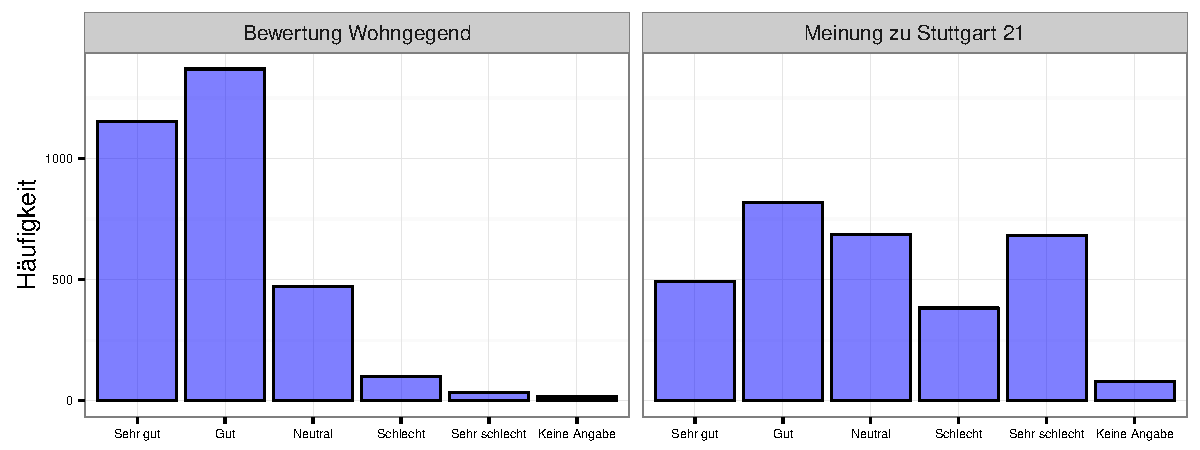
\includegraphics[scale=0.8]{Pictures/BarResp}
 \caption{Endogene Variablen}
 \label{endogene}
 \end{center}
\end{figure}

Aus Abbildung \ref{endogene} ist zudem ersichtlich, dass die Verteilungen der Beiden Variablen sehr verschieden sind für die gleichen Antwortmöglichkeiten. Während die meisten befragten Personen ihre Wohngegend mit \textit{Gut} oder \textit{Sehr gut} bewertet haben, sind die Antworten zum Projekt Stuttgart 21 eher gleichmäßig verteilt. Mögliche Ursachen für dieses Phänomen könnten sein, dass [..].\\
Für die exogen zu modellierenden Variablen sind detailliertere Informationen zu den Häufigkeiten der Ausprägungen im Anhang verfügbar. 


\subsection{Räumliche Effekte}



\section{Methodik}

\subsection{Modell}

\subsection{Modellwahl}

\subsection{Evaluierung}

\section{Ergebnisse}



%\clearpage
%============================================== Conlcusion =========================================================%

\section{Ergebnisse}

\clearpage


%============================================ References ===========================================================%
\addcontentsline{toc}{section}{\numberline{}Literatur}
\bibliographystyle{apalike}
\bibliography{} 

%\section{References}
%\renewcommand{\section}[2]{}
%\addcontentsline{toc}{section}{References}
%\renewcommand{\bibname}{4 References}
%\phantomsection
%\addcontentsline{toc}{section}{References}




\clearpage

%============================================== Appendix ============================================================%
%\appendix
%\pagestyle{Myheadings}
%\chead{APPENDIX}
%\pagestyle{}
%\section{$A^{-1}$ Appendix}
%\setcounter{secnumdepth}{0}

\begin{appendix}

\section*{Anhang}
\addcontentsline{toc}{section}{\numberline{}Anhang}


\begin{table}[h]
\centering
\caption{Grundgesamtheit Bürgerumfrage}
\adjustbox{max height=\dimexpr\textheight-5.5cm\relax,
           max width=\textwidth}{
\begin{tabular}{l|c|c}
\multicolumn{3}{l}{Anzahl Beobachtungen: 470.190}     \\ 
\hline \hline
\textbf{Variable} & \textbf{Skalenniveau} & \textbf{Anzahl Klassen}  \\ 
\multicolumn{1}{l|}{Altersklasse} &  Ordinal & 14 \\ \hline
\multicolumn{1}{l|}{Geschlecht} &  Nominal  & 2 \\ \hline
\multicolumn{1}{l|}{Nationalität} & Nominal  & 2 \\ \hline
\multicolumn{1}{l|}{Familienstand} & Nominal & 4 \\ \hline
\multicolumn{1}{l|}{Haushaltsgröße} &  Ordinal  & -- \\ \hline
\multicolumn{1}{l|}{Wohndauer} & Ordinal  & -- \\ \hline
\multicolumn{1}{l|}{ALG II Quote} & Ordinal  & 9 \\ \hline
\multicolumn{1}{l|}{Ein/Zweifamilienhäuser}& Ordinal & -- \\ \hline 
\multicolumn{1}{l|}{Gauß-Krüger} & Stetig Räumlich & \\ \hline \hline
\end{tabular}

}
\end{table}

\begin{table}[h]
\centering
\caption{Grundgesamtheit Zensus}
\adjustbox{max height=\dimexpr\textheight-5.5cm\relax,
           max width=\textwidth}{
\begin{tabular}{l|c|c}
\multicolumn{3}{l}{Anzahl Beobachtungen: 380.238}     \\ 
\hline \hline
\textbf{Variable} & \textbf{Skalenniveau} & \textbf{Anzahl Klassen}  \\ 
\multicolumn{1}{l|}{Altersklasse} &  Ordinal & 9 \\ \hline
\multicolumn{1}{l|}{Geschlecht} &  Nominal  & 2 \\ \hline
\multicolumn{1}{l|}{Nationalität} & Nominal  & 2 \\ \hline
\multicolumn{1}{l|}{Familienstand} & Nominal & 4 \\ \hline
\multicolumn{1}{l|}{Haushaltsgröße} &  Ordinal  & -- \\ \hline
\multicolumn{1}{l|}{Wohnfläche} & Ordinal  & 24 \\ \hline
\multicolumn{1}{l|}{Stellung Beruf} & Nominal  & 9 \\ \hline
\multicolumn{1}{l|}{Beamter}& Nominal & 2 \\ \hline 
\multicolumn{1}{l|}{Gebäudetyp}& Nominal & 10 \\ \hline
\multicolumn{1}{l|}{Gebäudenutzung}& Nominal & -- \\ \hline
\multicolumn{1}{l|}{Gauß-Krüger} & Stetig Räumlich & \\ \hline \hline
\end{tabular}

}
\end{table}

\begin{figure}[h]
 \begin{center}
 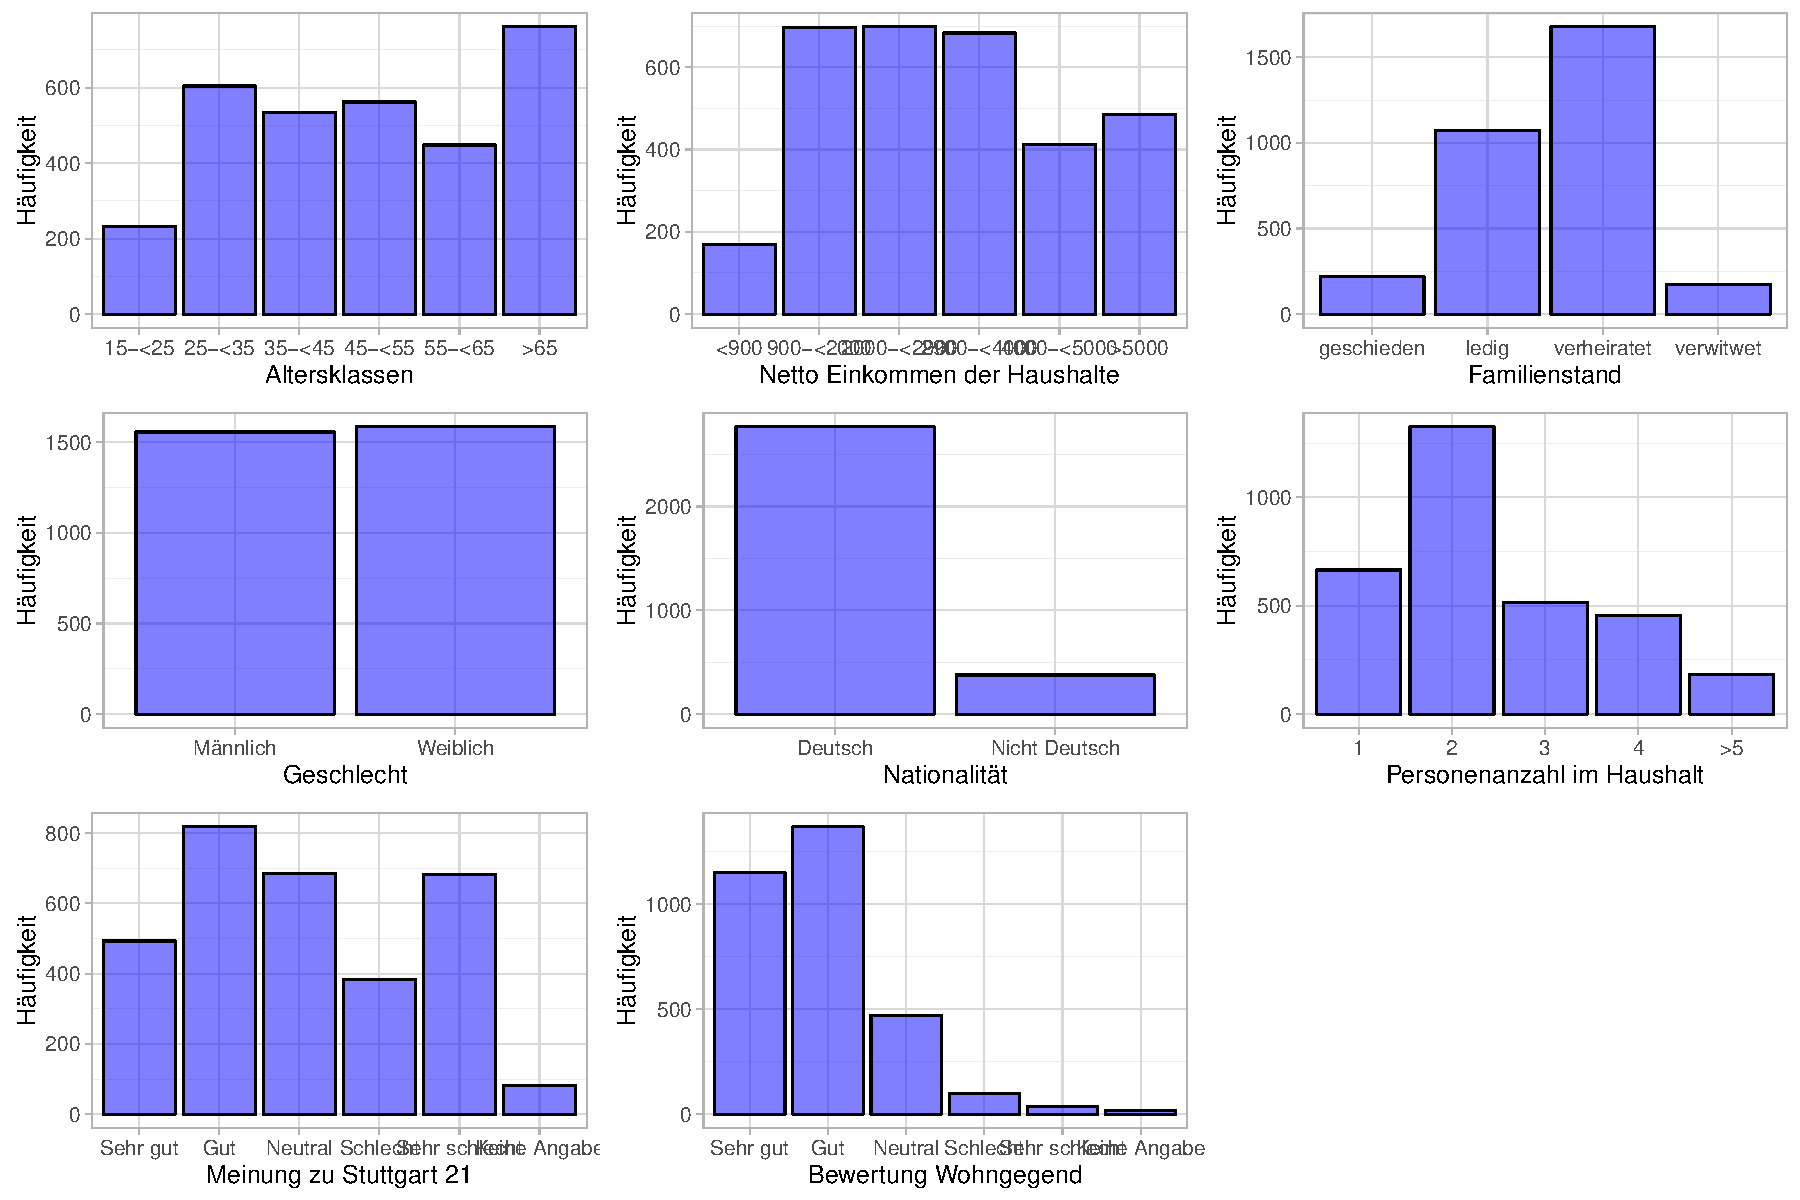
\includegraphics[scale=0.8]{Pictures/BarData}
 \end{center}
\end{figure}

\end{appendix}
\clearpage
\pagestyle{plain}
%\phantomsection
%\addcontentsline{toc}{section}{Eigenständigkeitserklärung}

%\section{Eigenständigkeitserklärung}

Hiermit versichere ich, dass ich die vorliegende Hausarbeit selbstständig verfasst und keine anderen als die angegebenen
Hilfsmittel benutzt habe. Alle wörtlich oder sinngemäß den Schriften anderer entnommenen Stellen
habe ich unter Angabe der Quellen kenntlich gemacht. Dies gilt auch für beigefügte Zeichnungen, Skizzen, bildliche
Darstellungen und dergleichen.\\
\\
Mir ist bewusst, dass ich mich im Falle einer unbeabsichtigten oder vorsätzlichen Missachtung durch den fehlerhaften
Umgang mit Quellen unter Umständen strafbar mache und die vorliegende Hausarbeit mit nicht ausreichend
bewertet wird.
\\
\\Göttingen, den
\\Unteschrift
\vspace*{4cm}
\\
Hiermit erlaube ich, dass meine Arbeit auf Betrug und falsche, sowie fehlende Zitate auch online geprüft wird.\\
\\
Mir ist bewusst, dass ich mich im Falle einer unbeabsichtigten oder vorsätzlichen Missachtung durch den fehlerhaften
Umgang mit Quellen unter Umständen strafbar mache und die vorliegende Hausarbeit mit nicht ausreichend
bewertet wird.
\\
\\Göttingen, den
\\Unterschrift
\clearpage


\end{document}
